\section{Learning side information with modality transfer}

\label{subsec:modality}

\begin{frame}{Proposed architecture}
	\vfill
	\begin{figure}
			\centering
			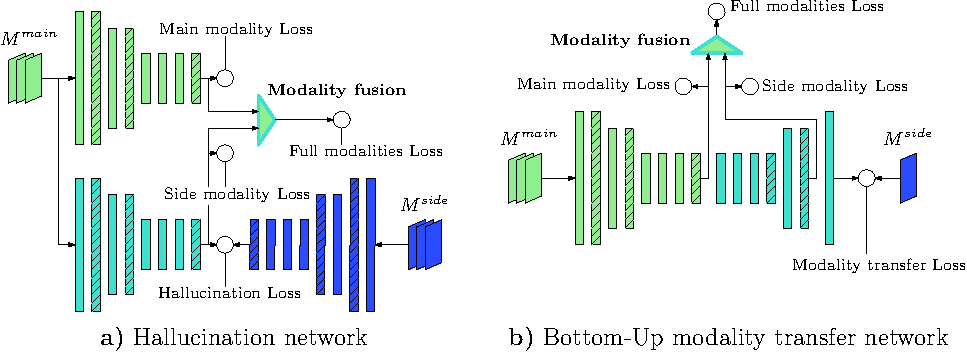
\includegraphics[width=0.48\linewidth, clip=true, trim = 8cm 0.5cm 0 0]{vect/training.pdf} \hfill
			\uncover<2>{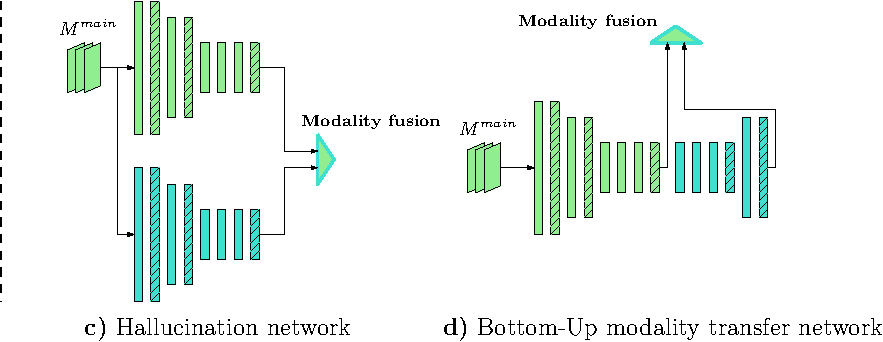
\includegraphics[width=0.48\linewidth, clip=true, trim = 7.6cm 0.5cm 0 0]{vect/testing.pdf}}
		\end{figure}
	\vfill
	The proposed architecture inspired by auto-encoder networks.
	\vfill
\end{frame}

\begin{frame}{Optimization}
	\begin{equation}
			Loss_{transfer} = \norm{\widetilde{M}(M^{main}) - M^{side}}^2,
	\end{equation}
	
	where $\widetilde{M}(x)$ denotes the output of the decoder part of the network regarding input $x$.
	
	\uncover<2->{	
	Final loss:
	\begin{multline}
			Loss = Loss_{triplet}^{main}*\sigma_{main} + Loss_{triplet}^{side}*\sigma_{side} \\
			+ Loss_{triplet}^{full}*\sigma_{full} + Loss_{transfer}*\sigma_{transfer}.
	\end{multline}
	}
	
	\uncover<3>{
	Diversification loss:
	\begin{equation}
		\label{eq:div_loss}
		Loss_{div} = min\left( Loss_{triplet}^{full} - Loss_{triplet}^{main} + \lambda_{div} , 0\right),
	\end{equation}
	where $\lambda_{div}$ is a scalar value that acts as a margin to ensure $Loss_{triplet}^{full}$ is always smaller than $Loss_{triplet}^{main}$.
	}
	
\end{frame}

\begin{frame}{Advantages over hallucination}
	Advantages of our bottom-up transfer approach (\textbf{BU-TF}) over hallucination network are threefold: 
	\begin{itemize}
		\item<2-> No need of pretraining on side modality
		\item<3-> Method by nature lighter: $29k$ parameters vs. $41k$ parameters for networks built upon Alexnet architecture
		\item<4> No need to transform modality into 3-channels data
	\end{itemize}
	

\end{frame}